\section{Ejercicio 3}

\subsection{Introducción}

\paragraph{}
El tercer y último ejercicio de este trabajo práctico, consistía en dado un modelo de una prisión decidir si una persona condenada podía escapar o no de la misma. Este modelo fue dado de tal manera que se pudiera representar utilizando un grafo. La idea general del modelo de esta prisión, fue que en la misma haya habitaciones y pasillos. Cada pasillo conectaba dos habitaciones y no había más de un pasillo conectando dos habitaciones. Además, cada habitación podía estar vacía, tener una puerta o tener una llave. Para pasar por una habitación que tuviera una puerta había que tener su respectiva llave.

\paragraph{}
Como requerimiento para este problema, se especificó que su solución debía tener una complejidad estrictamente menor que \Ode{n^3}, con n igual a la cantidad de habitaciones.


\subsection{Explicación}
\label{explicacion3}

\paragraph{}
En primer instancia, se pensó en alguna forma de recorrer el grafo de manera que la misma sirviera para solucionar el problema planteado. Inmediatamente, surgió la idea de utilizar el método BFS para dicho fin.

\paragraph{}
Seguidamente, se realizaron algunos ejemplos en papel, para ver de que forma se iba a comportar el método elegido para este modelo en cuestión, ya que se no podía utilizar un BFS normal por las restricciones con las que se contaba. Luego de observar este comportamiento, se encontró una forma de resolver el problema utilizando BFS, la cuál se explica a continuación.

\paragraph{}
La idea utilizada para este ejercicio resultó bastante simple. La misma consiste en los siguientes pasos:
\begin{itemize}
	\item Se comienza a realizar BFS desde la primer habitación.
	\item Cada vez que se encuentra una habitación con una llave, ésta se guarda en un conjunto de llaves.
	\item Cada vez que se encuentra una habitación con puerta pueden suceder 2 cosas:
	\begin{itemize}
		\item Si ya se había encontrado su llave, se la recorre como si no tuviese puerta.
		\item Si no se había encontrado su llave, se la ingresa a una cola donde se alojaran las habitaciones con estas características, sin aplicar BFS en ella.
	\end{itemize}
	\item Cuando el recorrido BFS termina, puede darse por dos motivos:
	\begin{itemize}
		\item Que se hayan recorrido todas las habitaciones.
		\item Que queden habitaciones sin recorrer en la cola de aquellas que tienen puerta y que cuando se las intentó visitar no se tenía su llave.
	\end{itemize}
\end{itemize}

Una vez terminado el primer BFS, se verifica si ya se recorrieron todas las habitaciones o, caso contrario, si quedan habitaciones que se puedan visitar\footnote{esto es equivalente a ver si de todas las habitaciones que quedaron encoladas por tener una puerta a la cuál no se tenía acceso, hay alguna de las que sí se tenga llave ahora}. Si sucede lo segundo, entonces se repiten todos los pasos antes mencionados tomando como primer habitación para recorrer con BFS alguna de las que se habían encolado de la cuál se tenga su llave.\\
Si sucede que se recorrieron todas las habitaciones o que no hay ninguna llave disponible que abra las habitaciones encoladas, entonces se sale de la recursión y se verifica si se visitó o no la última habitación (o habitación de salida). Si se visitó entonces significa que hay forma de salir de la prisión y sino, significa lo contrario.

\paragraph{}
A continuación se adjunta, a modo de pseudocódigo, los algoritmos utilizados para resolver el problema descrito anteriormente. En los mismos usaremos a \textit{n} como la cantidad de habitaciones (o nodos).


\SetKw{Orden}{Complejidad:}
\textbf{bool} resolver(carcel c)\\
\begin{algorithm}[H]
\Orden{\Ode{n^2}}\\

	
	$vector<bool>$ habitacionesYaVisitadas(c.cantHabitaciones)\tcp*{\Ode{n}}
	
	$queue<int>$ habitacionesLimites;
	
	$vector<bool>$ llavesEncontradas(c.cantHabitaciones)\tcp*{\Ode{n}}
	
	int proximaHabitacion;

	bool puedoSeguir = true\tcp*{\Ode{1}}
	
	int contador;
	
	bool termine = false\tcp*{\Ode{1}}
	
	proximaHabitacion = 0\tcp*{\Ode{1}}
	
	\While{(puedoSeguir $\wedge$ $\neg$termine)}{

		recorrerPorBFS(proximaHabitacion, habitacionesLimites, habitacionesYaVisitadas, llavesEncontradas, c)\tcp*{\Ode{n^2}}
		
		termine = habitacionesLimites.empty()\tcp*{\Ode{1}}
		
		\If{($\neg$termine)\tcp*{\Ode{1}}}{
		
			contador = habitacionesLimites.size()\tcp*{\Ode{1}}
			
			\While{(puedoSeguir $\&\&$ ($\neg$llavesEncontradas[habitacionesLimites.front()]))\tcp*{\Ode{n}}}{
				
				habitacionesLimites.push(habitacionesLimites.front())\tcp*{\Ode{1}}
				
				habitacionesLimites.pop()\tcp*{\Ode{1}}
				
				contador--\tcp*{\Ode{1}}
				
				\If{(contador == 0)\tcp*{\Ode{1}}}{puedoSeguir = false\tcp*{\Ode{1}}}
			}
			
			proximaHabitacion = habitacionesLimites.front()\tcp*{\Ode{1}}
			
			habitacionesLimites.pop()\tcp*{\Ode{1}}
			
			
		}	
	}

	\eIf{(habitacionesYaVisitadas[c.cantHabitaciones-1])\tcp*{\Ode{1}}}{return true}{return false}
\end{algorithm}


\textbf{void} recorrerPorBFS(int proximaHabitacion, $queue<int>\&$ habitacionesLimites, vector$<bool>\&$ habitacionesYaVisitadas, vector$<bool>\&$ llavesEncontradas, carcel$\&$ c)\\
\begin{algorithm}[H]
\Orden{\Ode{n^2}}\\
	$queue<int>$ habitacionesProximas
	
	habitacionesProximas.push(proximaHabitacion)
	
	habitacionesYaVisitadas[proximaHabitacion] = true\tcp*{\Ode{1}}
	
	int actual
	
	\While{(!habitacionesProximas.empty())\tcp*{\Ode{n}}}{
	
		actual = habitacionesProximas.front()\tcp*{\Ode{1}}
		
		habitacionesProximas.pop()\tcp*{\Ode{1}}
				
		\If{(c.tieneLlave(actual))\tcp*{\Ode{1}}}{
			llavesEncontradas[c.dameLlave(actual)] = true\tcp*{\Ode{1}}
		}
		
		\For{ (int i = 0; i$<$c.cantHabitaciones; i++)\tcp*{\Ode{n}}} {
	
			\If{(c.sonAdyacentes(actual,i) $\wedge$ $\neg$habitacionesYaVisitadas[i])\tcp*{\Ode{1}}}{
		
				\eIf{(c.tienePuerta(i) $\wedge$ $\neg$llavesEncontradas[i])\tcp*{\Ode{1}}}{
					habitacionesLimites.push(i)\tcp*{\Ode{1}}
				}{
					habitacionesProximas.push(i)\tcp*{\Ode{1}}
				}
				habitacionesYaVisitadas[i] = true\tcp*{\Ode{1}}
			}
		}
		
	}



\end{algorithm}



\subsection{Análisis de la complejidad del algoritmo}

\paragraph{}
Para el análisis de complejidad de los algoritmos que resuelven el problema dado, vamos a remitirnos a los pseudocódigos propuestos en la sección [\ref{explicacion3}]. Como aclaración, cabe decir que en los siguientes párrafos vamos a referirnos a \textit{n} como la cantidad de habitaciones en la prisión (cantidad de nodos del grafo).\\
En primer instancia vamos a analizar el pseudocódigo del algoritmo \textit{recorrerPorBFS}. La complejidad del mismo está dada por un flujo \textit{for} anidado dentro de otro flujo \textit{while}. Es visible que el flujo \textit{for} tiene una complejidad \titade{n} ya que todas las operaciones dentro suyo son de complejidad \Ode{1} y el mismo se ejecuta n veces. Quizás no sea tan claro por qué el flujo \textit{while} tiene complejidad igual a \Ode{n}. Esto se debe a la naturaleza del algoritmo BFS. En BFS se recorre cada nodo una única vez, y si vemos cuándo es que termina de ejecutarse dicho flujo, veremos que lo hace cuando se vacía la cola \textit{proximasHabitaciones}. Esta cola puede tener un largo de hasta n habitaciones (por lo dicho previamente sobre el método BFS) por lo que este flujo se ejecutará como máximo tantas veces como habitaciones haya.

\paragraph{}
Una vez realizado el análisis del algoritmo \textit{recorrerPorBFS} sólo nos queda verificar qué complejidad cumple el algoritmo \textit{resolver}. Si se observa con atención, puede notarse que la complejidad del mismo está dada por el llamado a la función \textit{recorrerPorBFS}. Pero no sólo basta con decir esto. También hay un flujo \textit{while} más adelante, el cuál solo tiene complejidad \Ode{n}. Esto se debe a que dicho flujo se va a ejecutar a lo sumo tantas veces como elementos haya en la cola \textit{habitacionesLimites}. Para saber cuántos elementos hay a lo sumo en esta cola debemos remitirnos a la función \textit{recorrerPorBFS} y ver que aquí sólo se alojaran aquellas habitaciones en las cuales haya una puerta de la que no se tenga la llave correspondiente. Por esto podemos ver que claramente en esta cola habrá a lo sumo n habitaciones.\\
Sólo basta una aclaración para que la complejidad de este algoritmo quede completa y ésta hace referencia al flujo \textit{while} que engloba a los flujos antes descritos. En un primer acercamiento, uno podría decir que este ciclo se ejecuta a lo sumo n veces, arrojando una complejidad de \Ode{n}, haciendo que la complejidad total sea \Ode{n^3} si recordamos que este engloba a una llamada a \textit{recorrerPorBFS} cuya complejidad había resultado ser \Ode{n^2}. Pero en realidad, si se mira más detalladamente se puede observar que este flujo va a ejecutarse tantas veces como haga falta para que \textit{recorrerPorBFS} pase por todos las habitaciones (o nodos), es decir, si por ejemplo en el primer llamado a la función \textit{recorrerPorBFS} se pasa por todos los nodos, entonces el ciclo en cuestión va a ejecutarse una única vez. Este análisis entonces nos permite ver que en este algoritmo, la complejidad esta dada por la de la función antes mencionada. En conclusión, la complejidad del algoritmo es \Ode{n^2}.

\subsection{Detalles de implementación}

\paragraph{}
Para compilar el programa sólo hace falta ejecutar el comando make en consola.

\paragraph{Modo de Uso}
En consola, utilizar el comando: \texttt{./3\_ej [entrada] [salida]}.\\
Los parámetros ``entrada'' y ``salida'' son opcionales. Si no se los utiliza, el programa toma por default los archivos ``Tp2Ej3.in'' como entrada y ``Tp2Ej3NUESTRO.out'' como salida. En el caso que se los utilice, se le deben pasar 2 nombres de archivos de entrada y salida respectivamente. El archivo de entrada debe existir y debe tener un formato válido, es decir, debe tener el formato descrito en el enunciado de este trabajo práctico. El archivo de salida puede existir o no. En caso de existir, este será completamente sobreescrito.


\subsection{Resultados}
\label{resultados3}
\paragraph{}
Para poder analizar el comportamiento del algoritmo propuesto como solución al problema dado fue necesario encontrar una forma de generar de manera automática grafos que lo modelen. Esto resulta de una gran dificultad y se torna mucho más complicado si se quieren generar grafos que lo modelen y que además cumplan con ciertas características. Por lo tanto, para generar los casos de prueba se recurrió a un método que utilice números aleatorios. Esto no nos permite elegir de manera flexible alguna característica particular para el modelo final, pero facilita mucho la construcción del generador automático.

\paragraph{}
Luego de realizar un análisis sobre el comportamiento de los algoritmos \textit{resolver} y \textit{recorrerPorBFS} notamos que en general siempre se van a obtener resultados similares. Para ello se realizaron distintas pruebas: 
\begin{itemize}
  \item Se generaron casos en los que la primer habitación estuviese conectada con la última. Esta se realiza debido a que ambos algoritmos dejan de iterar si, entre otras condiciones, ya se visitó la última habitación.
  \item Para otros casos, se puso la restricción que ninguna habitación podía estar conectada con la última. Esto significa que no había solución posible.
  \item Por último, se generaron casos completamente azarosos, con la única precaución que la primer y última habitación no estuviesen unidas entre sí (de otra forma, esto sería igual al primer item).
\end{itemize}

\paragraph{}
Cabe aclarar que para los casos en los que se analizó el tiempo que necesitaba la implementación para resolver el problema, se hicieron varias corridas por cada caso y luego se tomó un promedio del tiempo total. Esto se realizó para evitar en mayor medida algún outlier que pudiera aparecer por cualquier evento ajeno al algoritmo.

\paragraph{}
Finalmente, del análisis antes realizado se desprenden algunas hipótesis, las cuales enunciaremos a continuación:
\begin{enumerate}
  \item Para los casos en los cuales no exista una comunicación directa entre la habitación 1 y la n-ésima, el algoritmo va a presentar una complejidad cuadrática.
  \item En los casos en que exista un pasillo que comunique directamente la primer habitación con la última, el algoritmo debería arrojar una complejidad lineal.
  \item En aquellos casos azarosos, la complejidad debería ser cuadrática pero en promedio será posible acotarla por una función lineal.
\end{enumerate}

\paragraph{}
A continuación presentamos los gráficos provenientes de las pruebas realizadas:

%	\begin{table}[t] %ubicacion de la tabla
%		\centering %centra la tabla
%		\begin{tabular}{c}
%			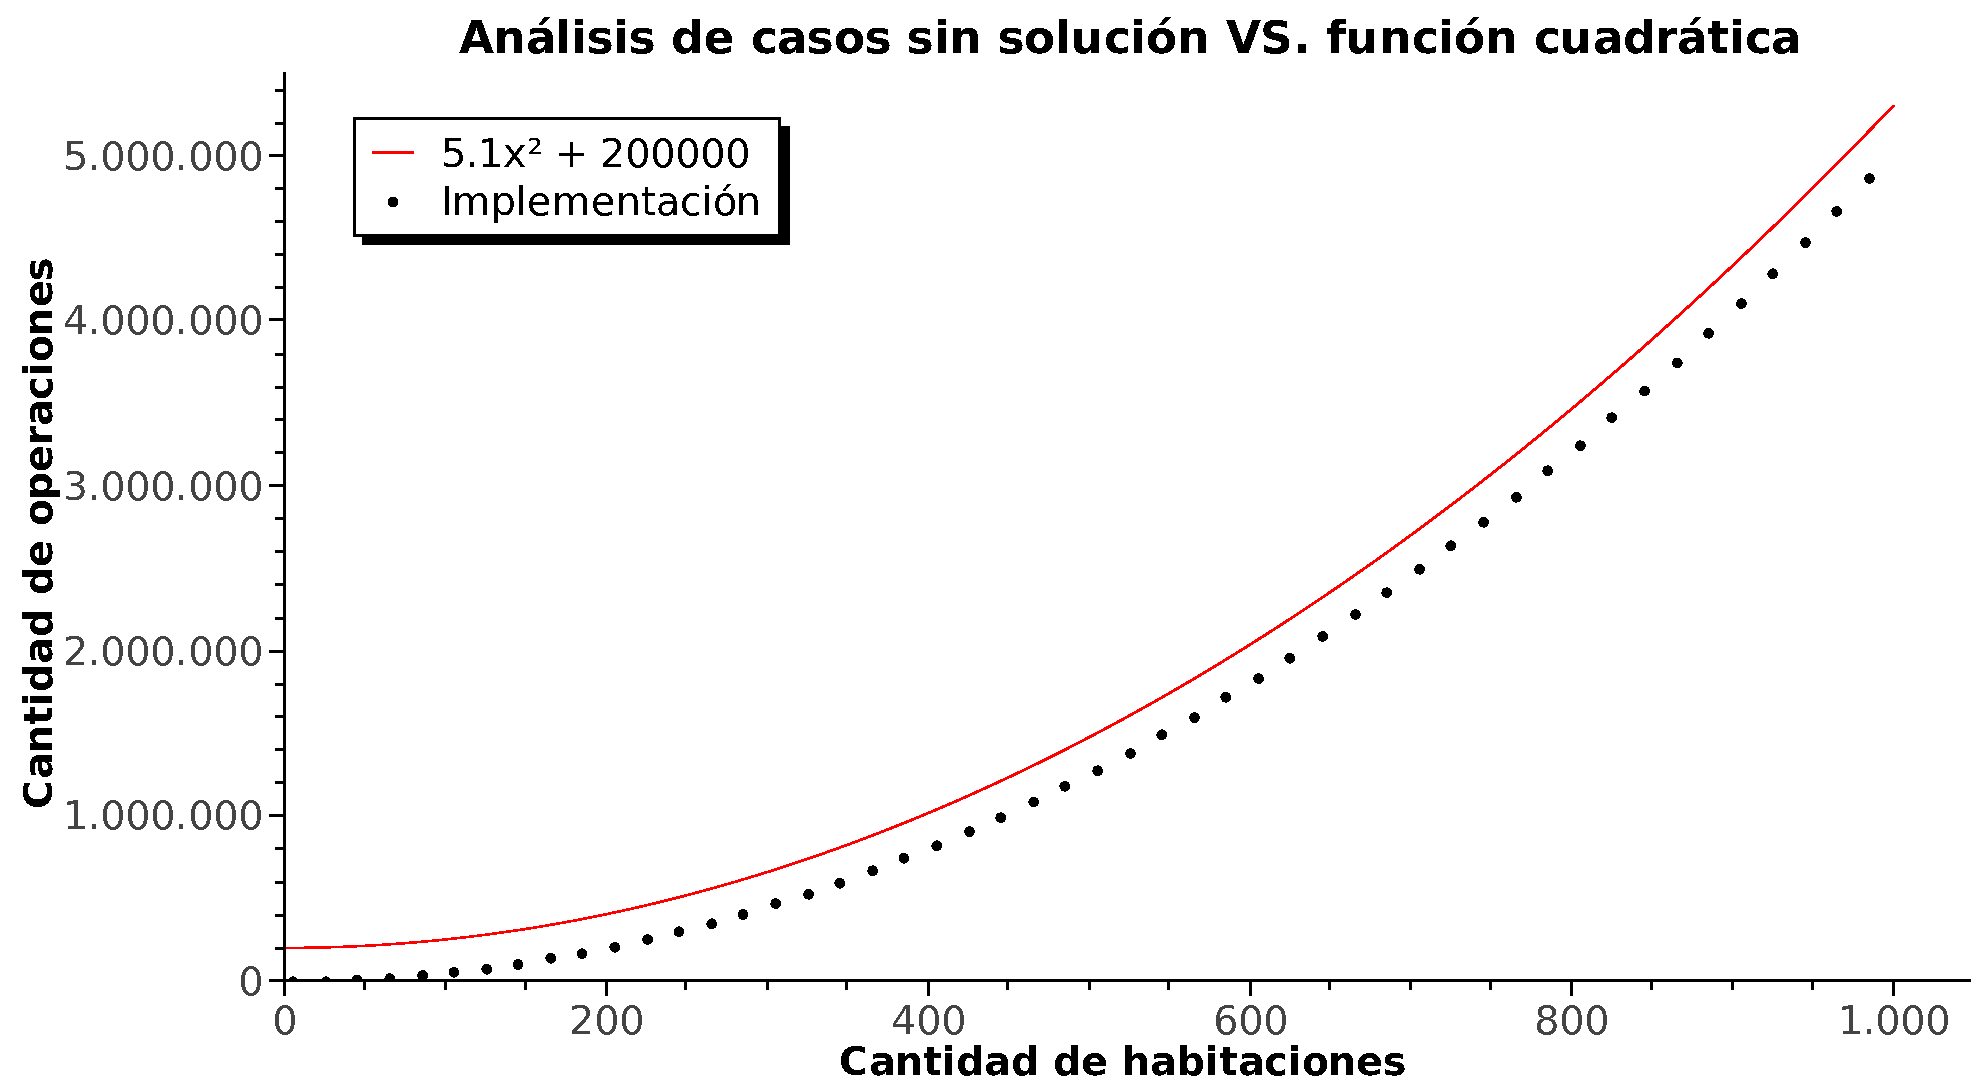
\includegraphics[scale=0.5]{../ej3/graficos/3_ej_contarOperacionesC.pdf} \\
%			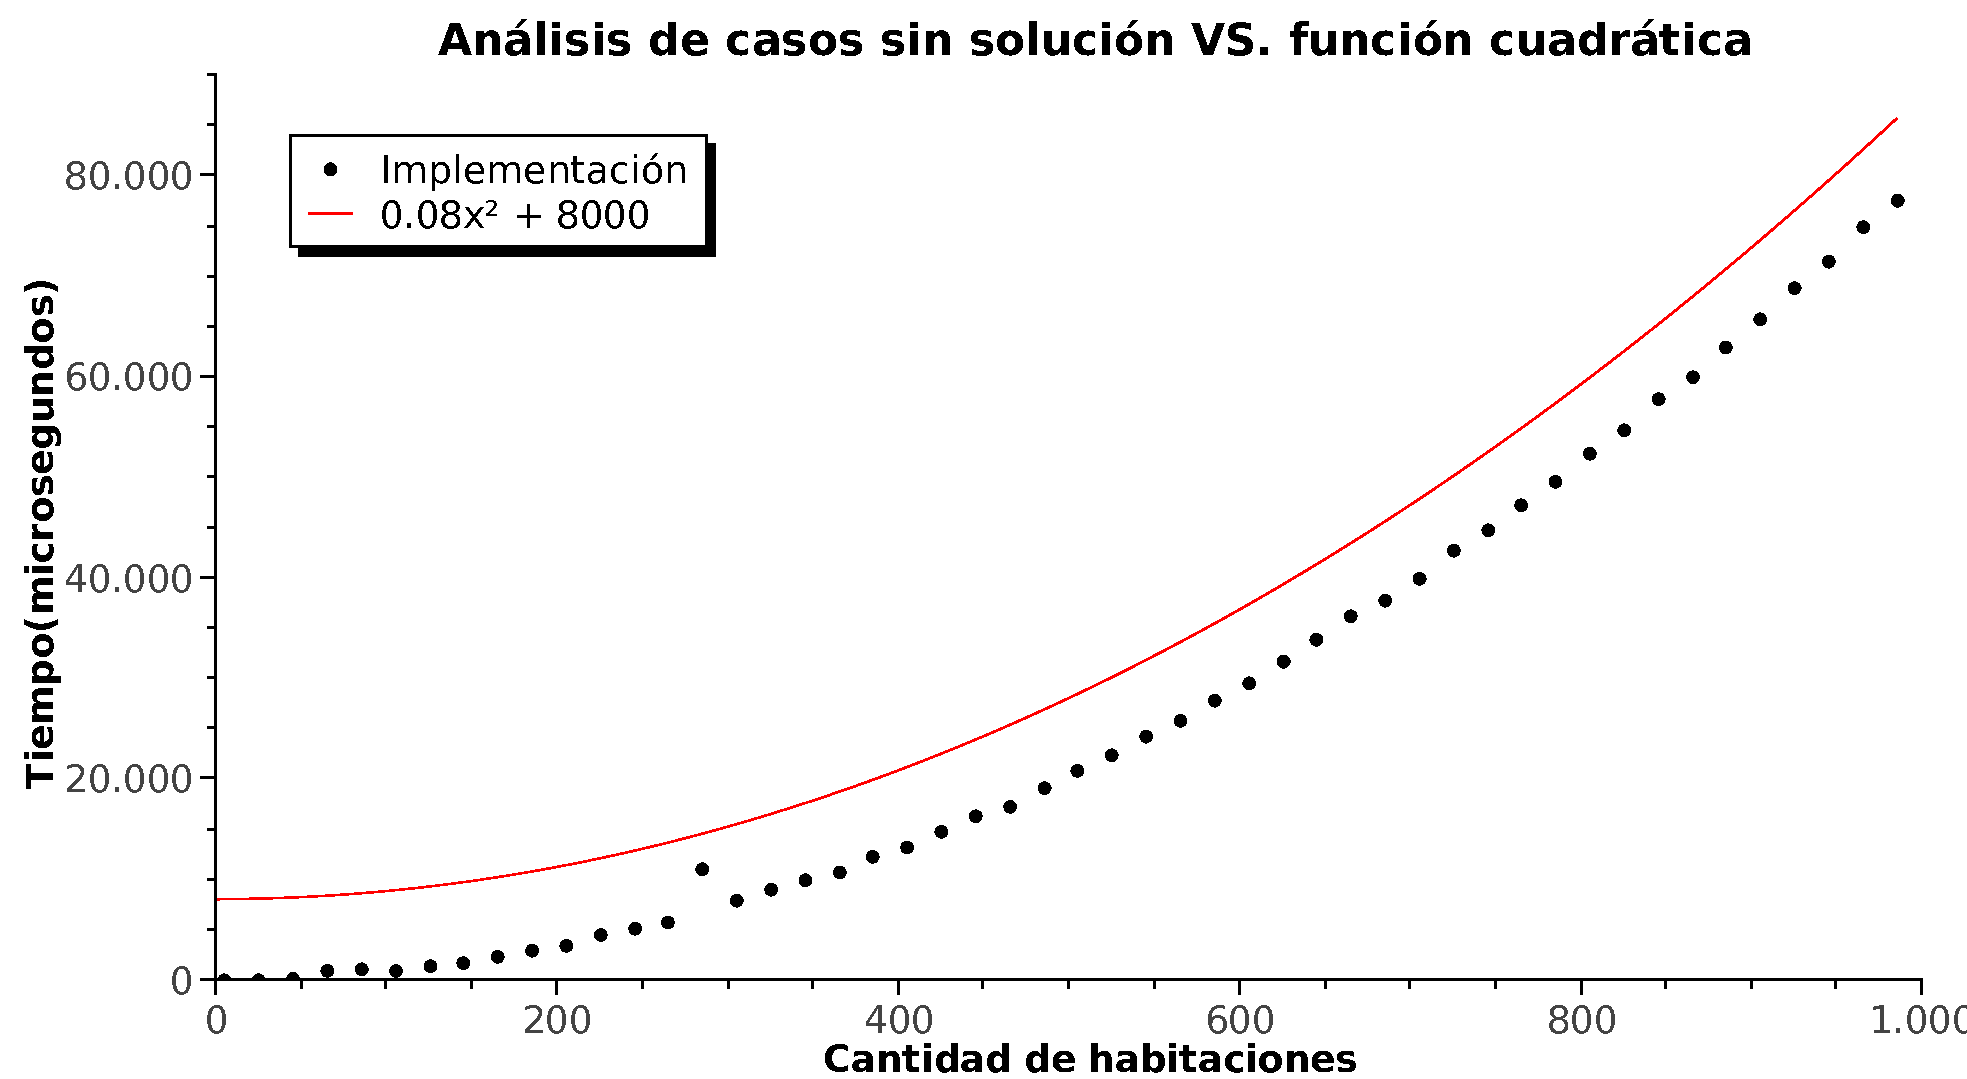
\includegraphics[scale=0.5]{../ej3/graficos/3_ej_contarTiempoC.pdf}
%		\end{tabular}
%		\caption{Muestran el comportamiento de la cantidad de habitaciones contra la cantidad de operaciones y contra el tiempo respectivamente. Las entradas fueron creadas de modo que no exista un resultado posible, es decir, que ninguna habitación este conectada con la última.} %titulo de la tabla
%		\label{3contarC} %con esto puedo referenciar a la tabla
		
%	\end{table}

%	\begin{table}[b] %ubicacion de la tabla
%		\centering %centra la tabla
%		\begin{tabular}{c}
%			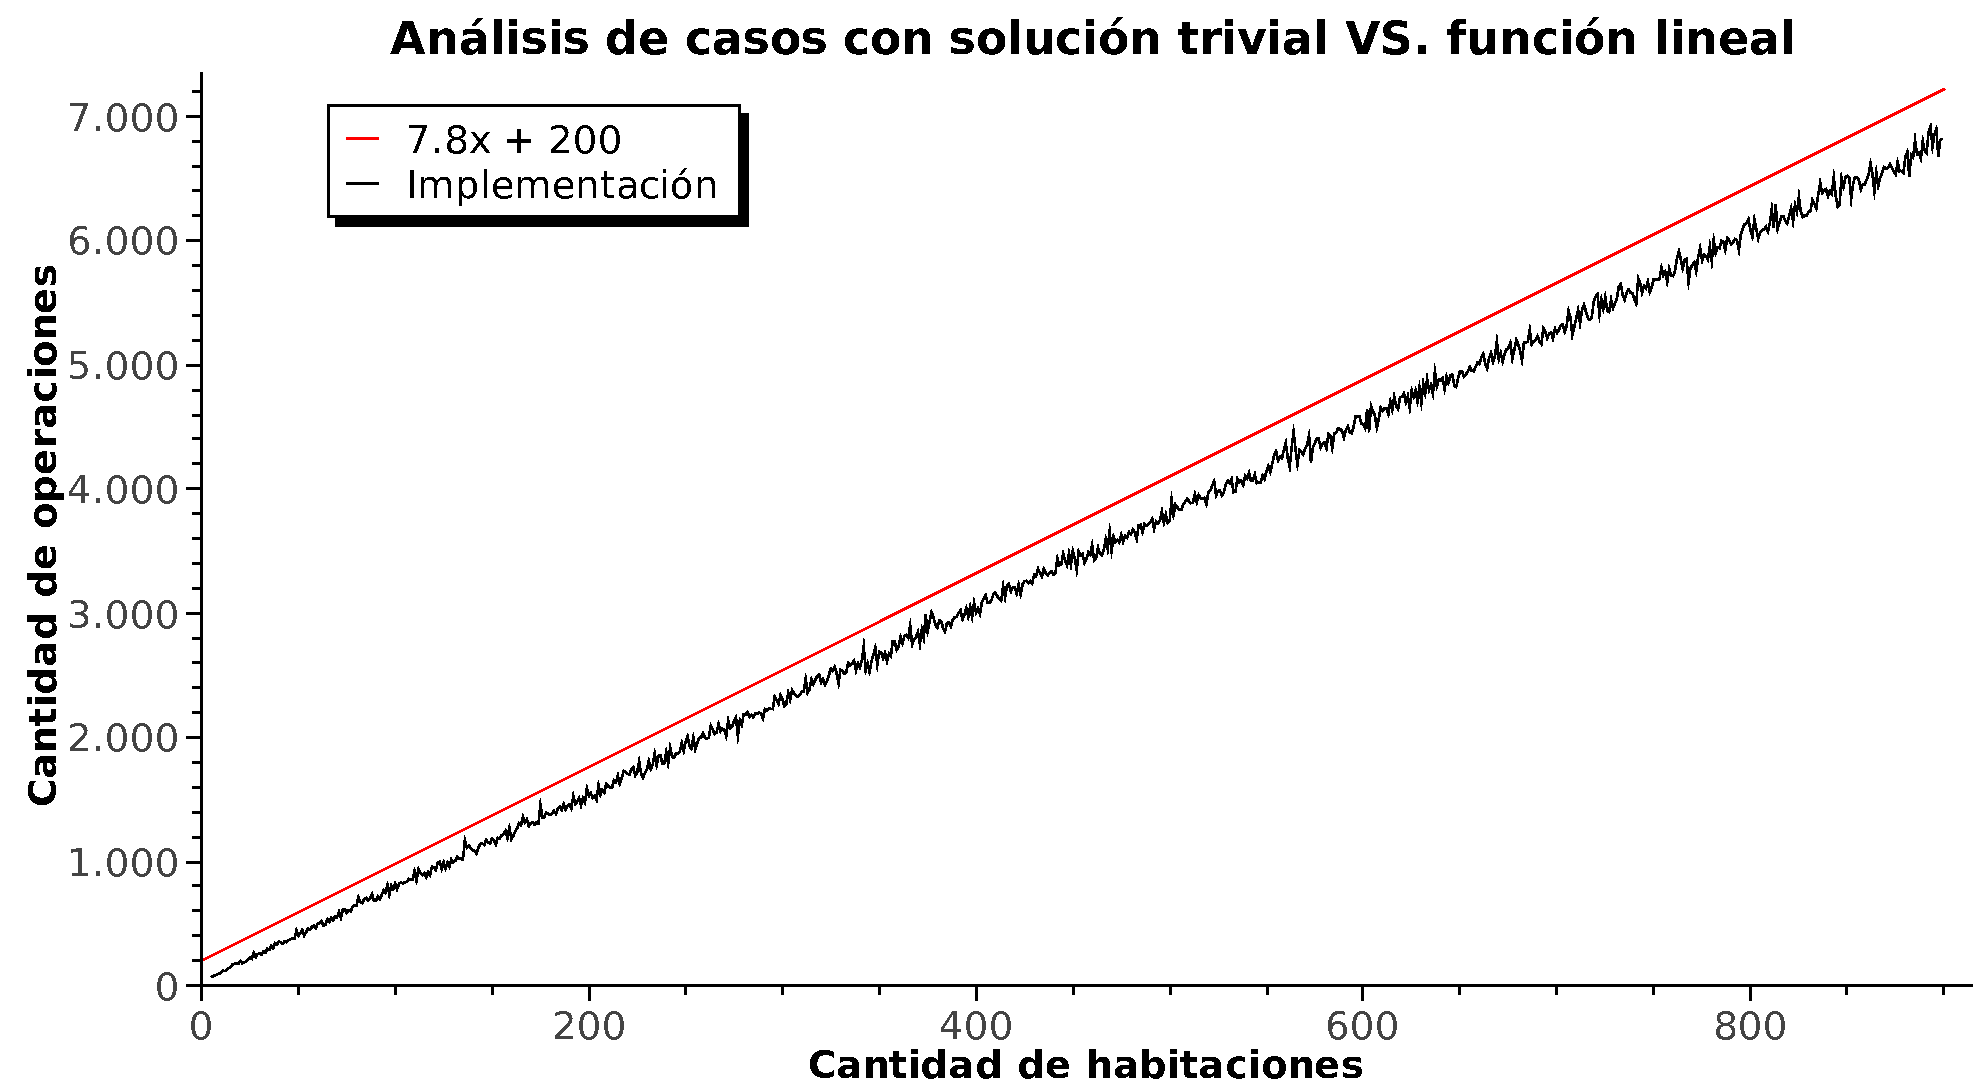
\includegraphics[scale=0.5]{../ej3/graficos/3_ej_contarOperacionesL.pdf} \\
%			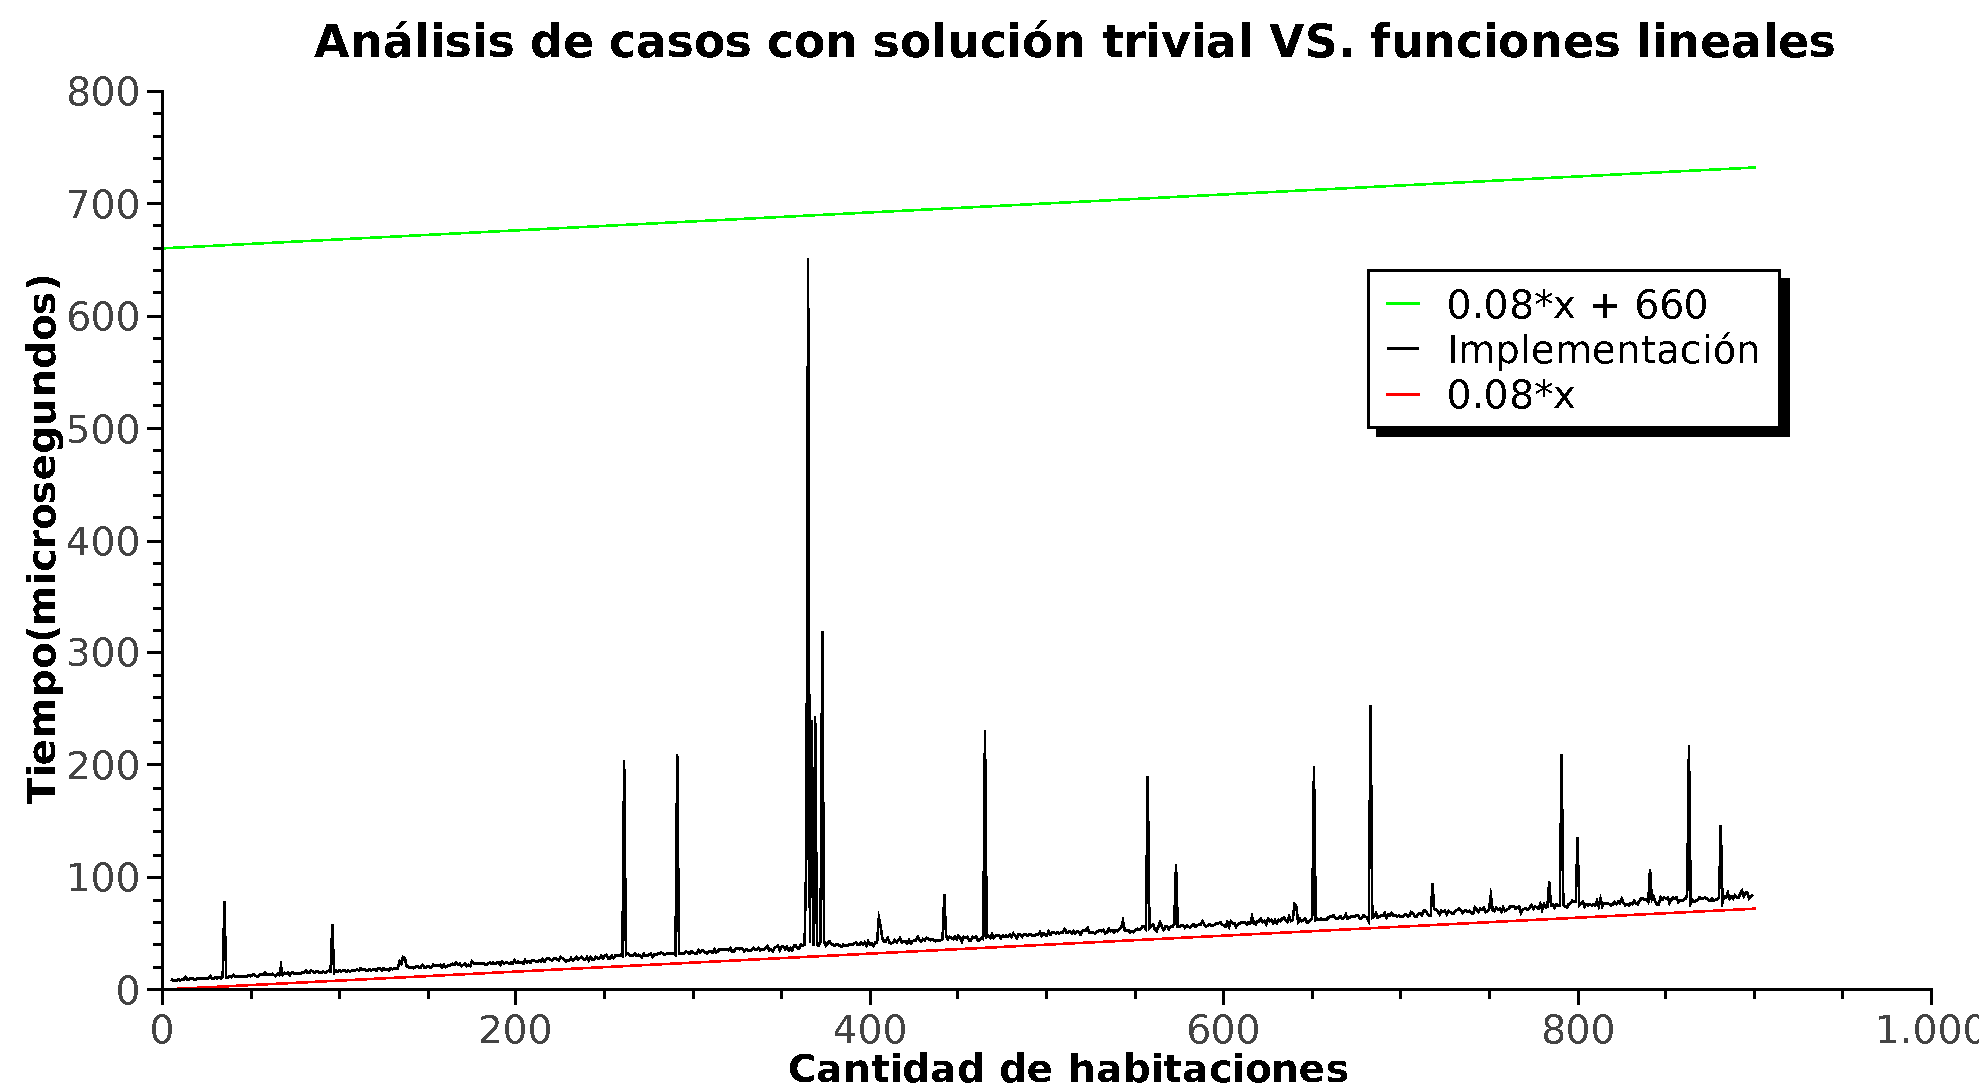
\includegraphics[scale=0.5]{../ej3/graficos/3_ej_contarTiempoL.pdf}
%		\end{tabular}
%		\caption{Muestran el comportamiento de la cantidad de habitaciones contra la cantidad de operaciones y contra el tiempo respectivamente. Las entradas fueron creadas de modo que haya un resultado trivial, es decir, que la primer habitación este conectada con la última.} %titulo de la tabla
%			\label{3contarL} %con esto puedo referenciar a la tabla \ref{Tiempo metodos}
%	\end{table}

%	\begin{table}[t] %ubicacion de la tabla
%		\centering %centra la tabla
%		\begin{tabular}{c}
%			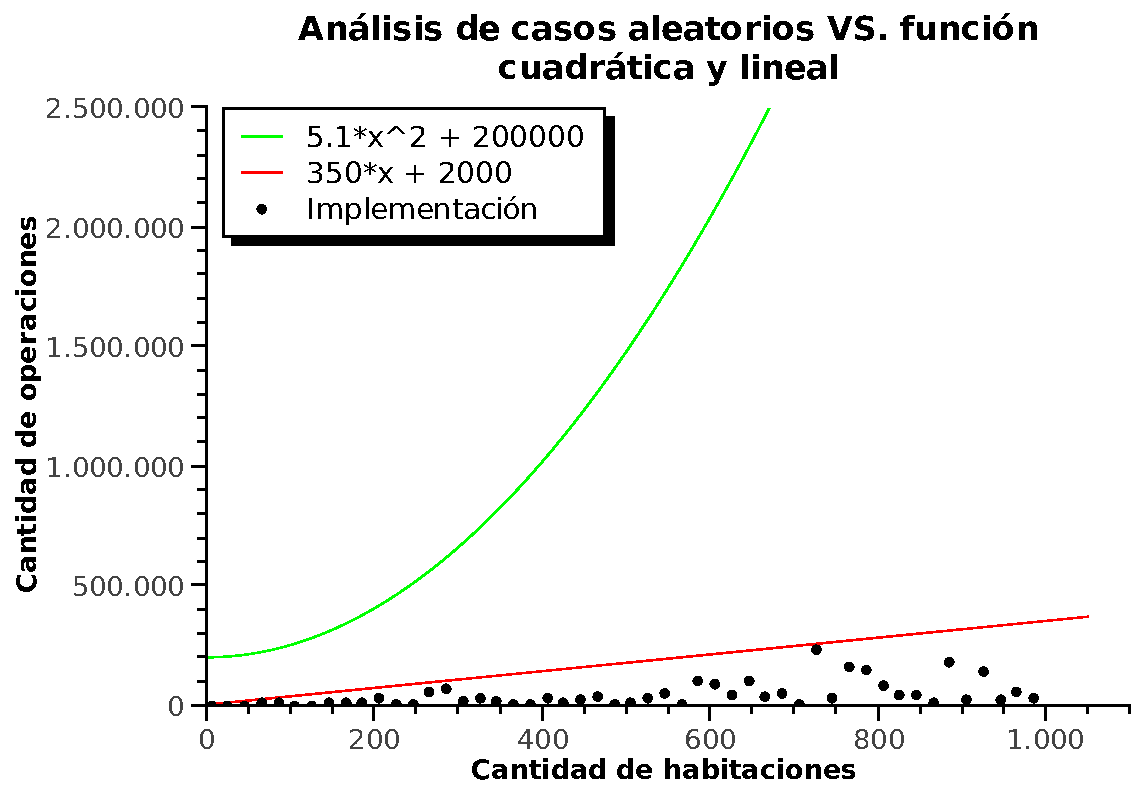
\includegraphics[scale=0.5]{../ej3/graficos/3_ej_contarOperacionesP.pdf} \\
%			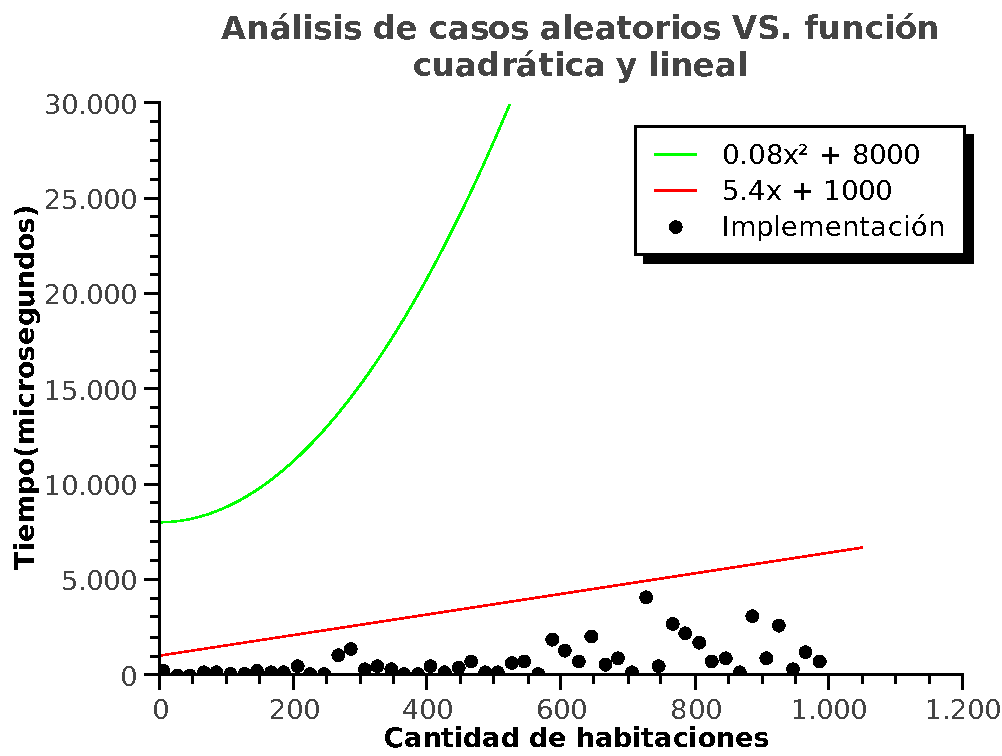
\includegraphics[scale=0.5]{../ej3/graficos/3_ej_contarTiempoP.pdf}
%			\end{tabular}
%		\caption{Muestran el comportamiento de la cantidad de habitaciones contra la cantidad de operaciones y contra el tiempo respectivamente. Las entradas fueron creadas al azar pero sin que exista un resultado trivial.} %titulo de la tabla
%		\label{3contarP} %con esto puedo referenciar a la tabla \ref{Tiempo metodos}
%	\end{table}

%primeras 2 imagenes
\begin{figure}[htb]
    \begin{minipage}{\textwidth}
	\begin{center}
		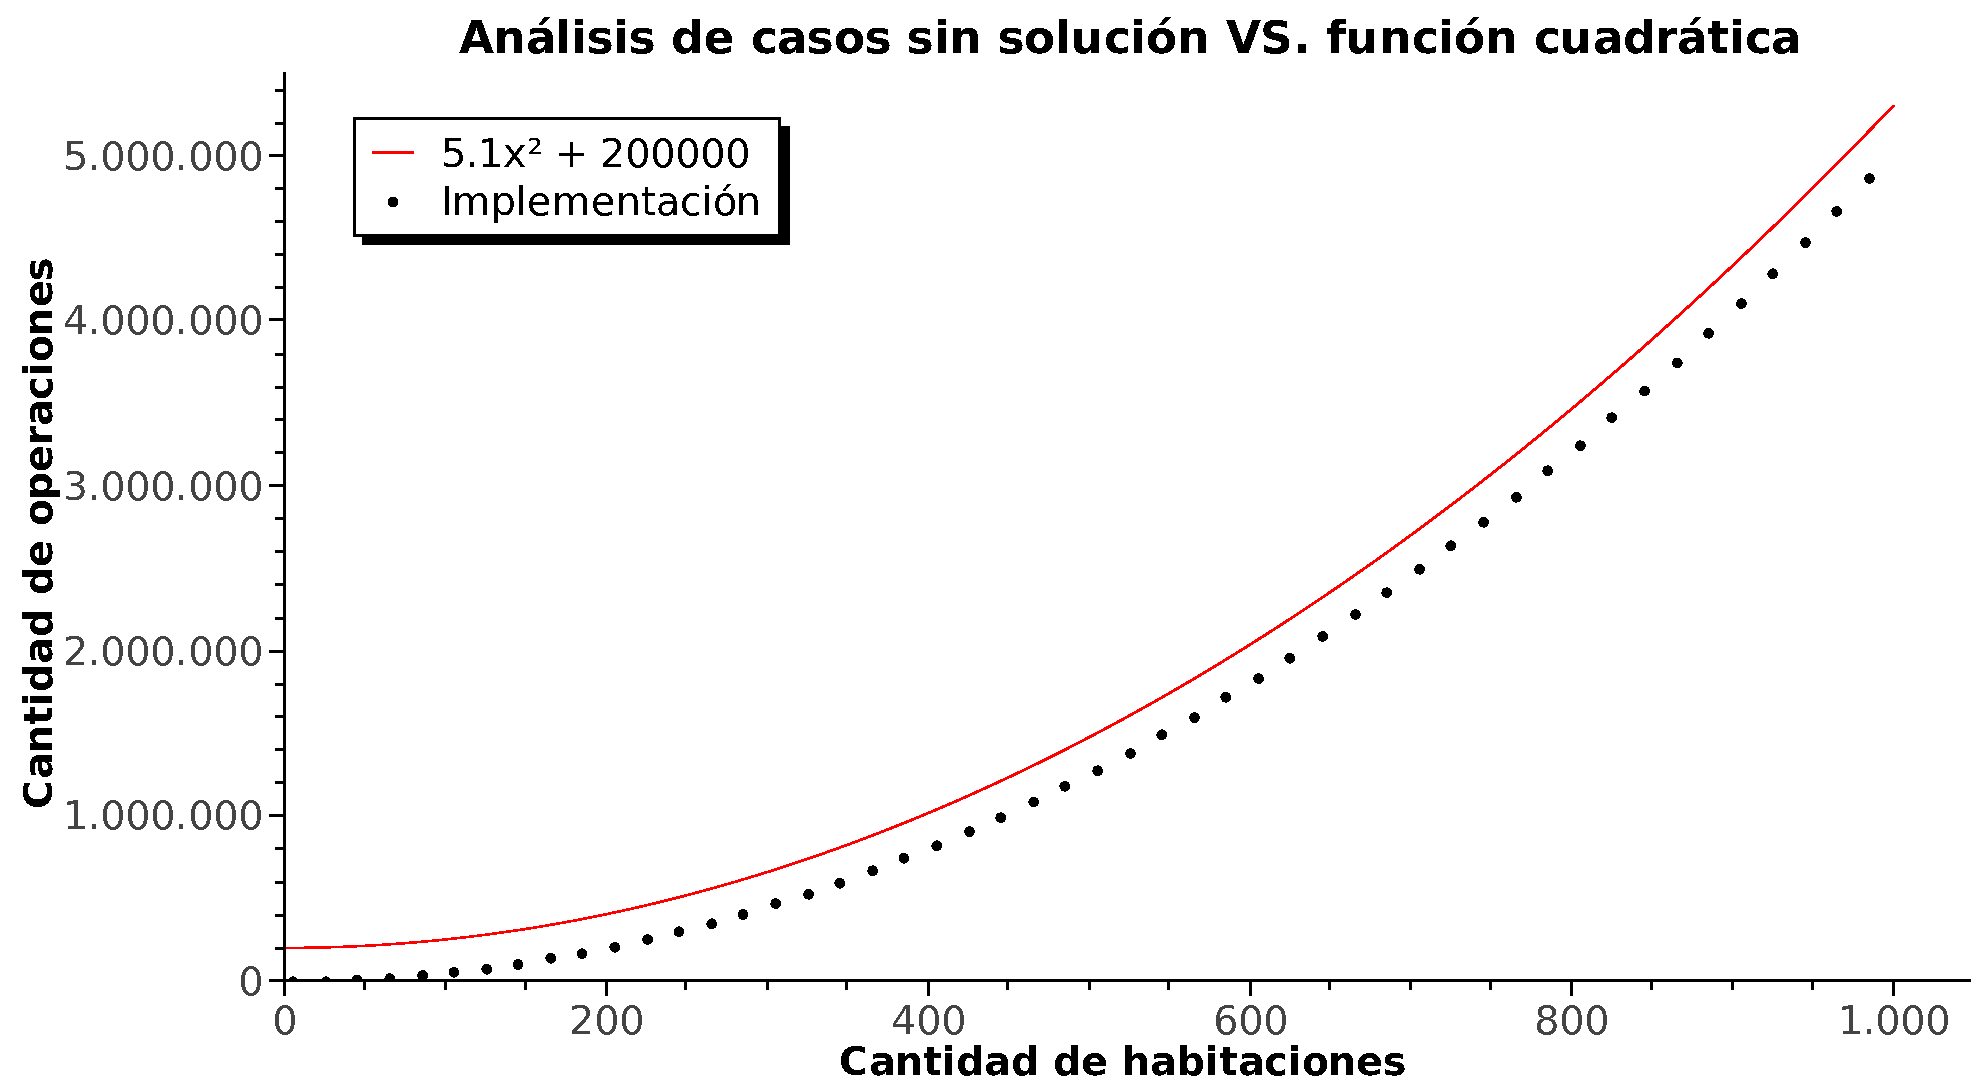
\includegraphics[width=\textwidth]{../ej3/graficos/3_ej_contarOperacionesC.pdf}
		\caption{Muestra el comportamiento del algoritmo comparando cantidad de habitaciones contra cantidad de operaciones. Las entradas fueron creadas de modo que no exista un resultado posible, es decir, que ninguna habitación este conectada con la última.}
		\label{3contarOpC}
	\end{center}
    \end{minipage}

    \begin{minipage}{\textwidth}
	\begin{center}
		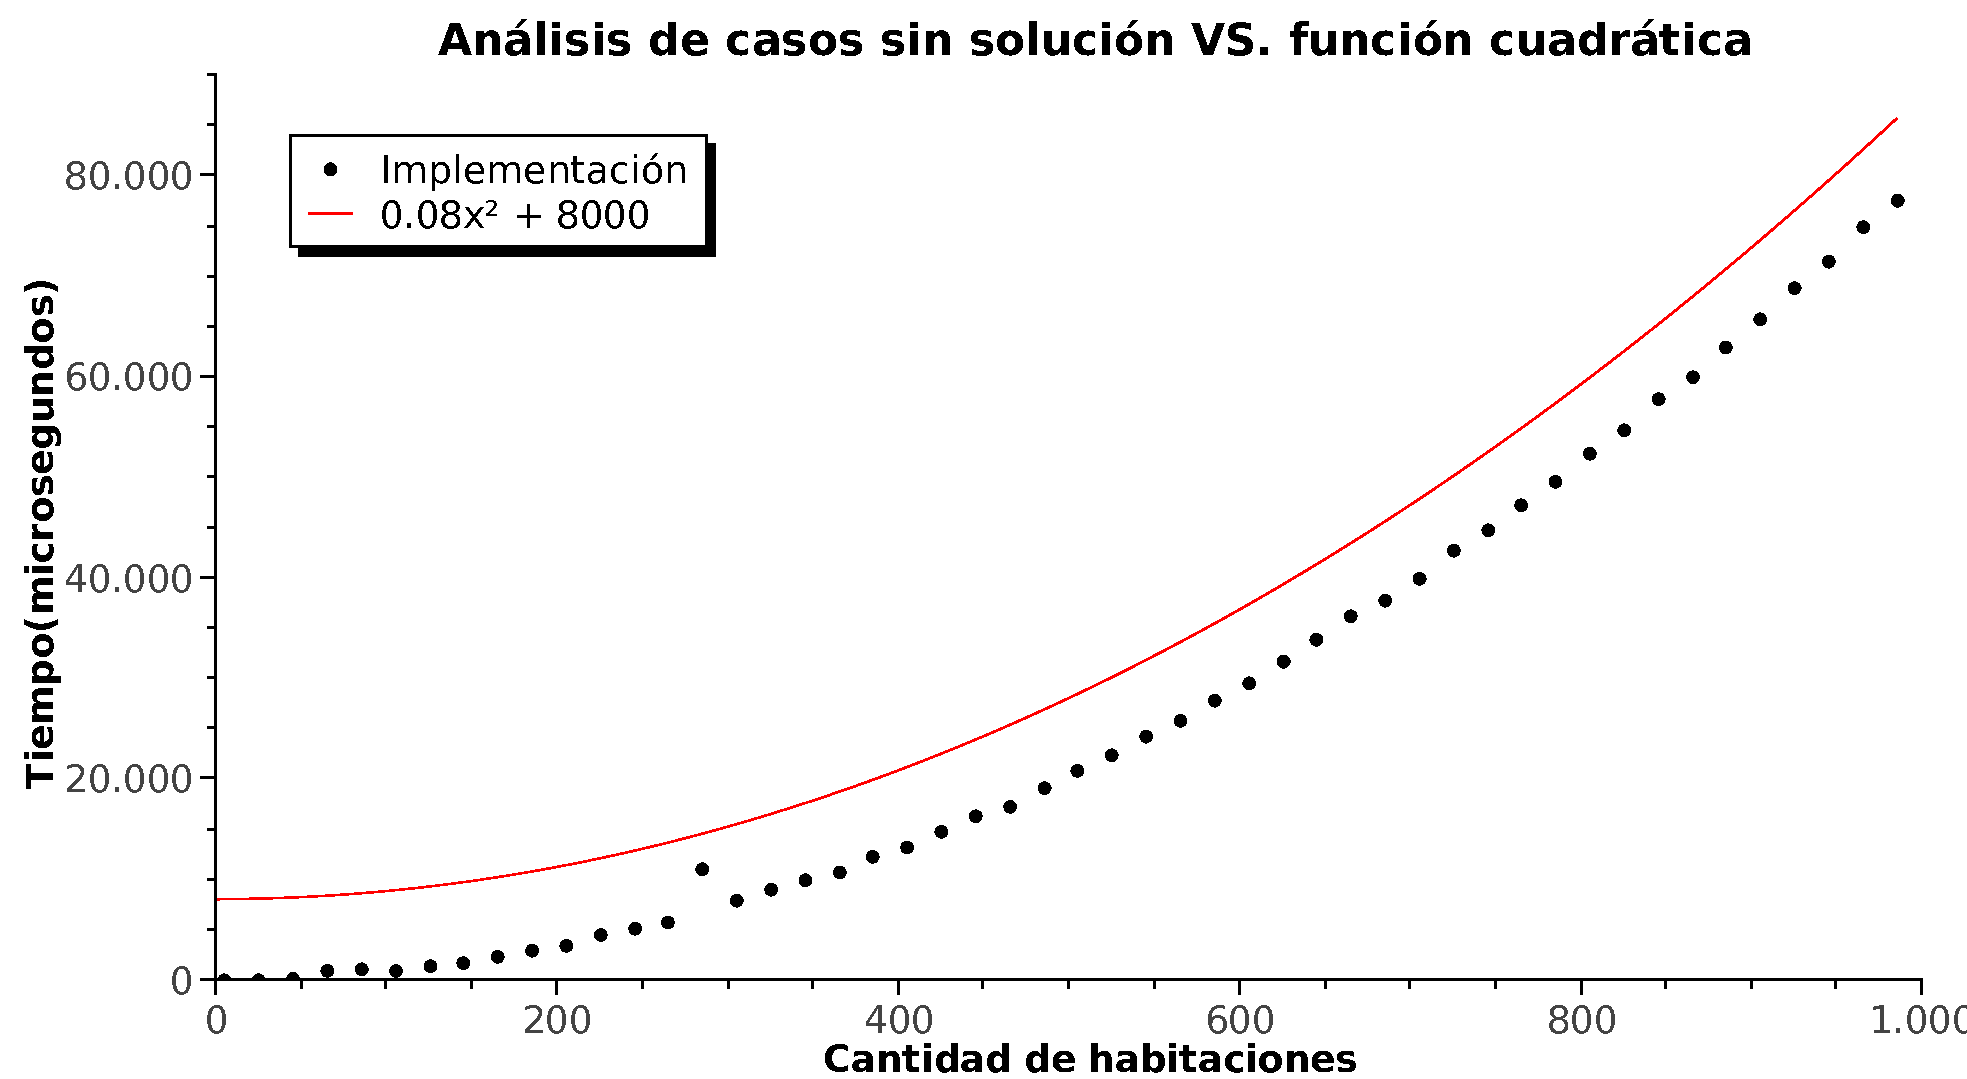
\includegraphics[width=\textwidth]{../ej3/graficos/3_ej_contarTiempoC.pdf}
		\caption{Muestra el comportamiento del algoritmo comparando cantidad de habitaciones contra tiempo de resolución. Las entradas fueron creadas del mismo modo que en la figura (\ref{3contarOpC}).}
		\label{3contarTiempoC}
	\end{center}
    \end{minipage}

\end{figure}

%segundas dos imagenes

\begin{figure}[htb]
    \begin{minipage}{\textwidth}
	\begin{center}
		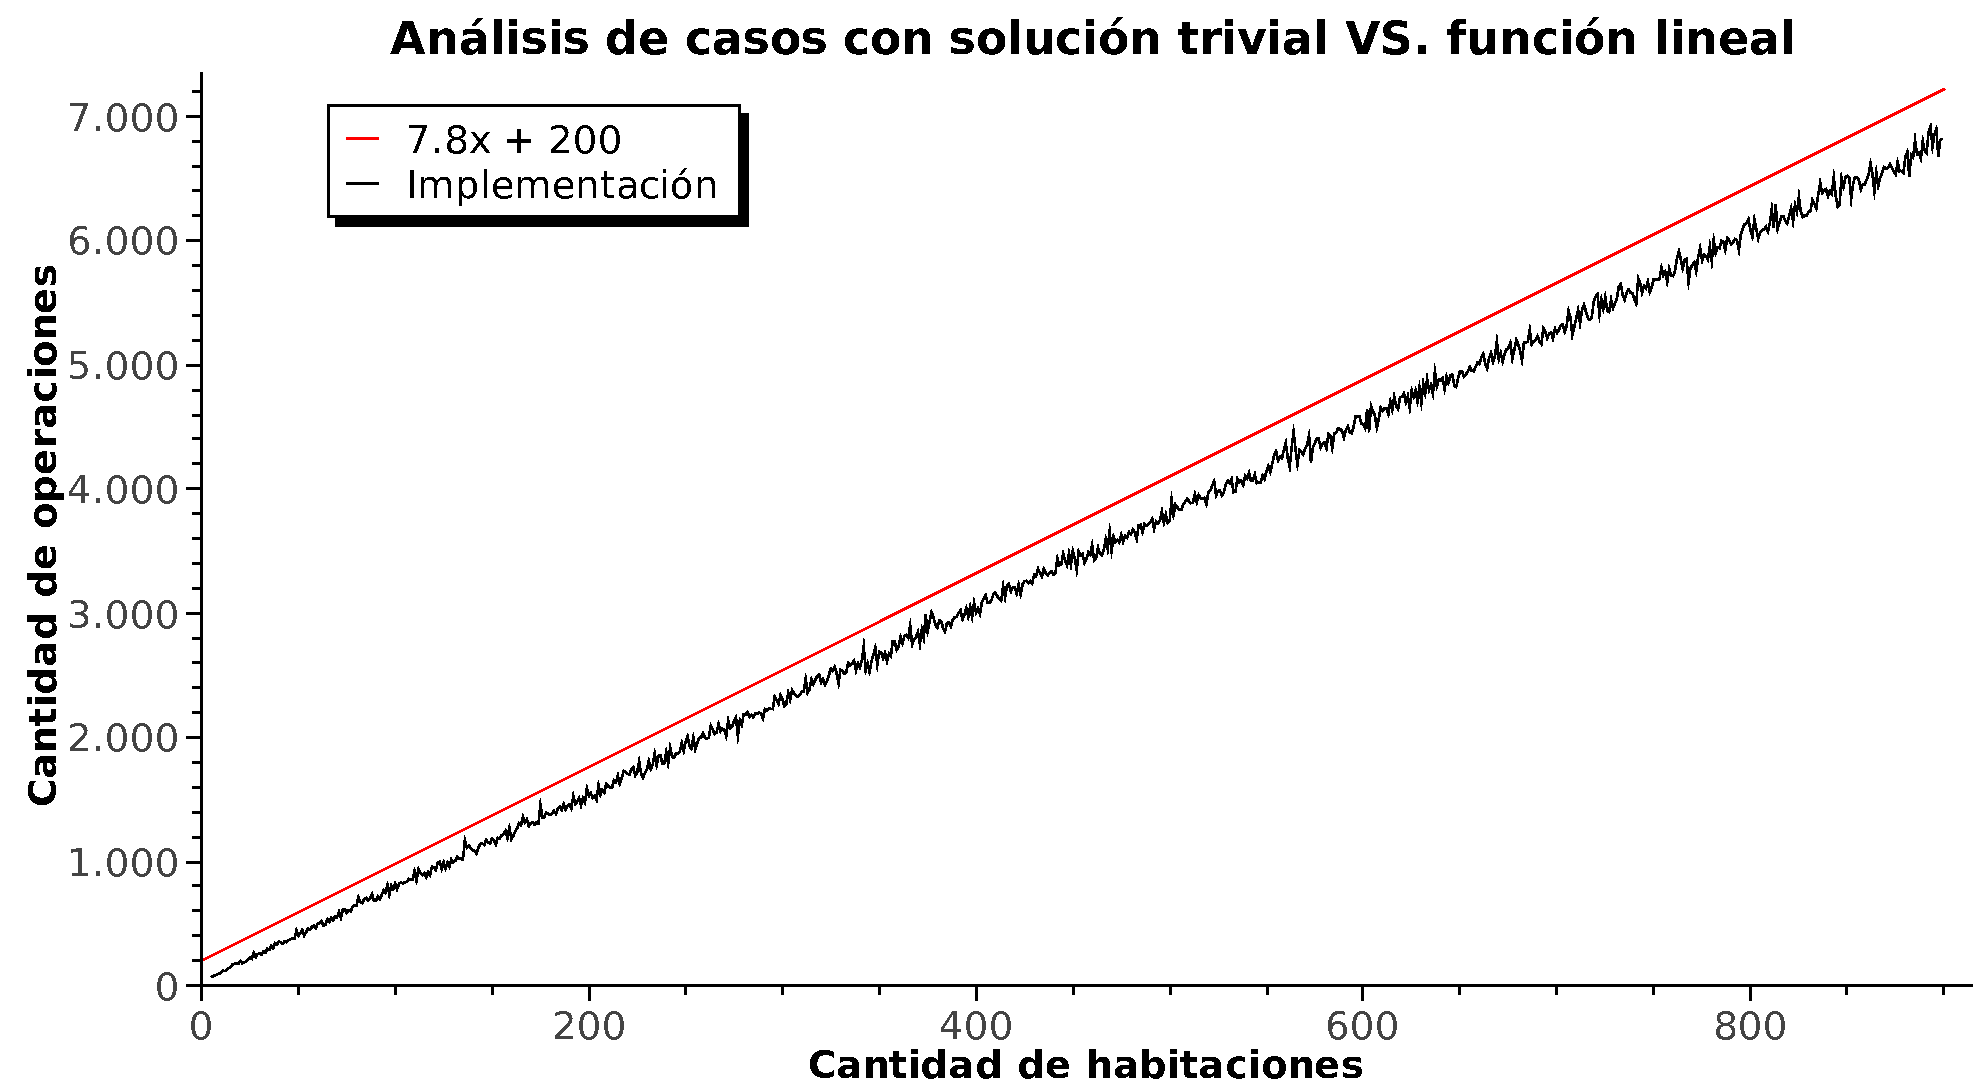
\includegraphics[width=\textwidth]{../ej3/graficos/3_ej_contarOperacionesL.pdf}
		\caption{Muestra el comportamiento del algoritmo comparando cantidad de habitaciones contra cantidad de operaciones. Las entradas fueron creadas de modo que exista un resultado trivial, es decir, que la primer habitación este conectada con la última.}
		\label{3contarOpL}
	\end{center}
    \end{minipage}

    \begin{minipage}{\textwidth}
	\begin{center}
		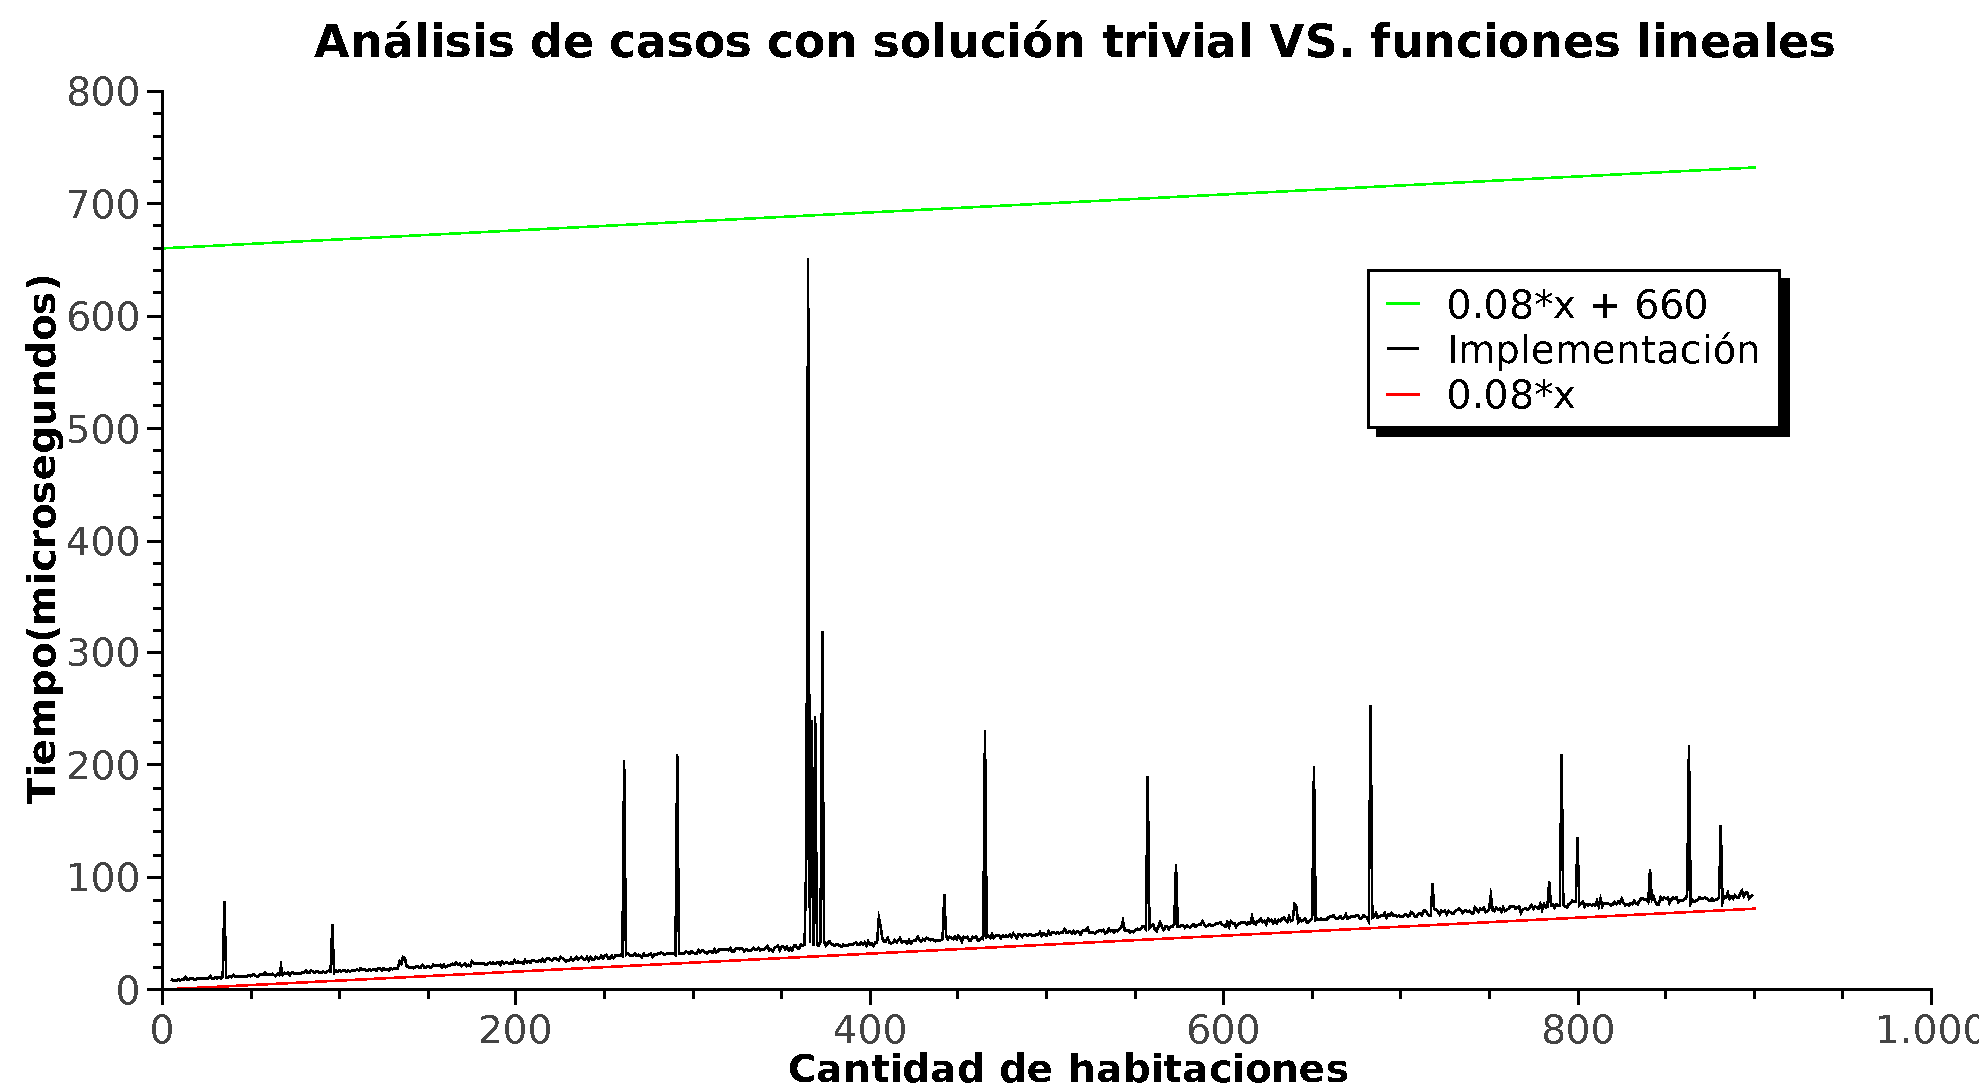
\includegraphics[width=\textwidth]{../ej3/graficos/3_ej_contarTiempoL.pdf}
		\caption{Muestra el comportamiento del algoritmo comparando cantidad de habitaciones contra cantidad de operaciones. Las entradas fueron creadas del mismo modo que en la figura (\ref{3contarOpL}).}
		\label{3contarTiempoL}
	\end{center}
    \end{minipage}

\end{figure}

%terceras dos imagenes

\begin{figure}[htb]
    \begin{minipage}{\textwidth}
	\begin{center}
		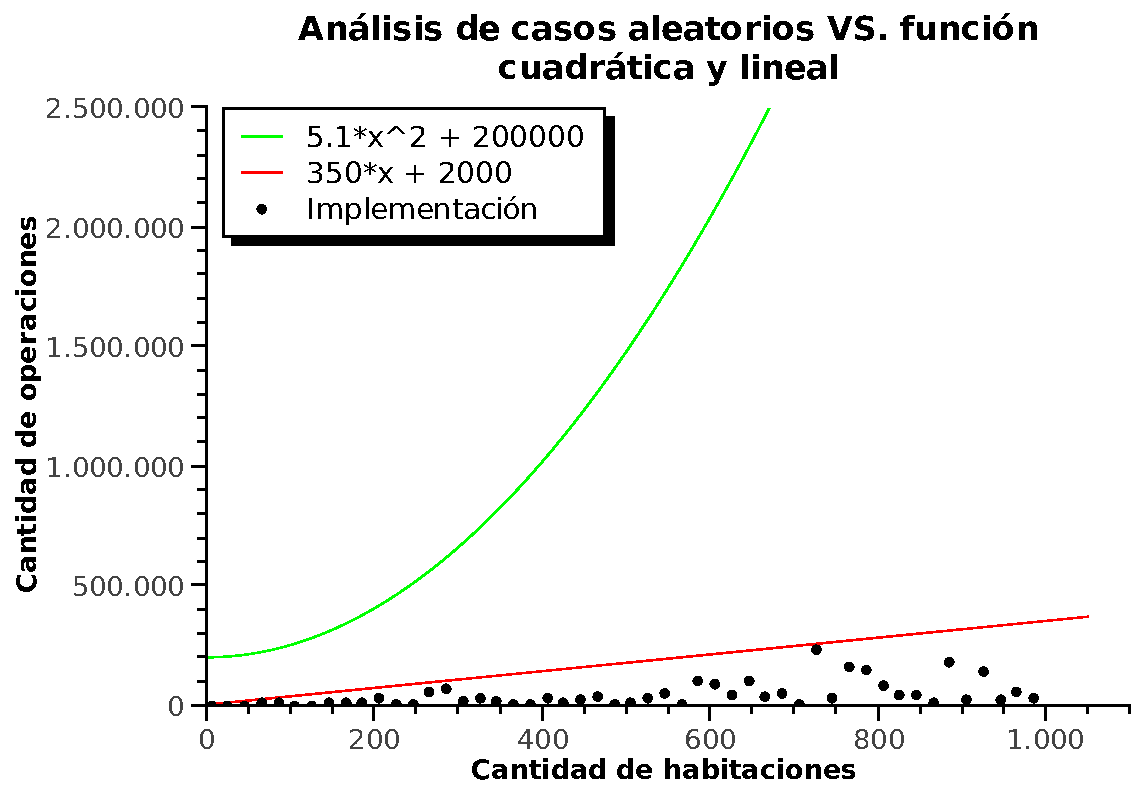
\includegraphics[width=\textwidth]{../ej3/graficos/3_ej_contarOperacionesP.pdf}
		\caption{Muestra el comportamiento del algoritmo comparando cantidad de habitaciones contra cantidad de operaciones. Las entradas fueron creadas al azar pero de modo que no exista un resultado trivial, es decir, que la primer habitación no estuviera conectada con la última.}
		\label{3contarOpP}
	\end{center}
    \end{minipage}

    \begin{minipage}{\textwidth}
	\begin{center}
		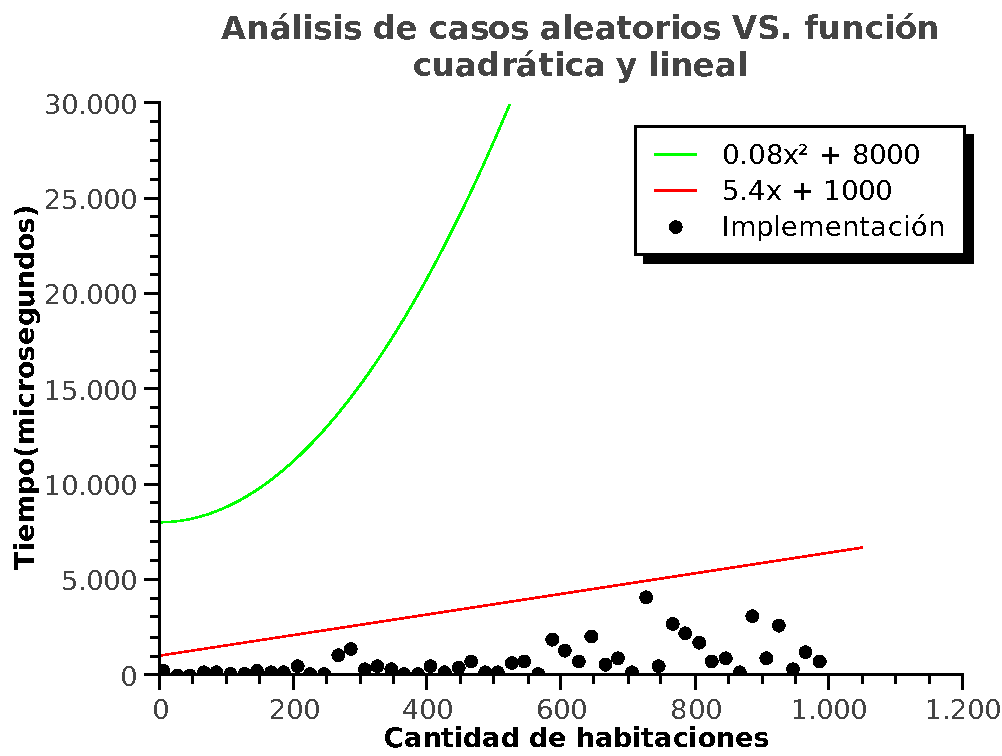
\includegraphics[width=\textwidth]{../ej3/graficos/3_ej_contarTiempoP.pdf}
		\caption{Muestra el comportamiento del algoritmo comparando cantidad de habitaciones contra cantidad de operaciones. Las entradas fueron creadas del mismo modo que en la figura (\ref{3contarOpP}).}
		\label{3contarTiempoP}
	\end{center}
    \end{minipage}

\end{figure}


\subsection{Debate}

\paragraph{}
De los resultados adjuntos en la sección anterior podemos observar algunos comportamientos particulares del algoritmo.\\
En los gráficos provenientes de los casos generados sin solución, se puede notar gran similitud entre los resultados arrojados durante la ejecución de la implementación y una función cuadrática. Esto puede deberse a que el algoritmo necesariamente va a recorrer todas las habitaciones posibles hasta concluir que no se visitó la última.

\paragraph{}
En el análisis de casos en los que hay una solución trivial, es decir en aquellos en los que la primer y última habitación son vecinas, los resultados tanto de tiempo como de cantidad de operaciones de la implementación parecieran estar acotados por una función lineal. Este comportamiento podría remitirse a cómo está implementado el algoritmo, en el cuál una vez que se visita a la última habitación no se continúan evaluando otras opciones sino que simplemente se devuelve un resultado positivo.

\paragraph{}
Por último tenemos aquellos casos en los que la disposición de las habitaciones y pasillos estaba totalmente realizada al azar salvo porque se ``prohibía'' la solución trivial. En estos gráficos se puede notar una disposición menos uniforme de los resultados provenientes de la implementación. Aquí se observa cómo estos pudieron ser acotados también por una función lineal.


\subsection{Conclusiones}

\paragraph{}
Si realizamos un análisis general de todo lo referente a este problema, podemos sacar algunas conclusiones. En general, en todos los casos de prueba que se analizaron, la implementación se comportó como se esperaba.\\
Se ve claramente cómo en el caso de las pruebas realizadas sobre entradas que no tenían solución, el algoritmo debe realizar muchas más operaciones que en los demás casos, ya que sólo deja de ejecutarse cuando se recorrieron todas las habitaciones alcanzables desde la primera. La cantidad de operaciones crece polinomialmente en comparación a la cantidad de habitaciones totales y por lo tanto también lo hace el tiempo que demora el algoritmo. Esto se debe a la forma en que se comporta el método BFS, cuya complejidad es \Ode{n^2}, con n igual a la cantidad de nodos del grafo (en este caso, a la cantidad de habitaciones). Por esto, podemos decir que la primer hipótesis realizada fue correcta.

\paragraph{}
En el caso de la segunda hipótesis, pasa algo similar a lo anterior. Esta hace referencia al comportamiento del algoritmo cuando se utilizan entradas que contienen una solución trivial. En este contexto, es claro que por el modo de operar de la implementación, se encuentra una solución ni bien se analizan todas las habitaciones vecinas a la primera, ya que entre ellas se encuentra la última. Por lo tanto, es fácil ver aquí que el peor caso se da cuando la primer habitación está conectada con todas (este es el peor caso en este contexto, es decir, en el que existe solución trivial). Esto puede observarse además en los gráficos de la sección [\ref{resultados3}], donde los datos arrojados por la implementación son claramente acotados por una función lineal.

\paragraph{}
En última instancia, no podríamos decir que la tercer hipótesis fue corroborada, ya que para ello se debería realizar un análisis mucho más complejo y teórico sobre los datos de entrada, y esto excede los fines de este trabajo práctico. Sin embargo, sí se pudo comprobar que para todos los casos analizados los resultados fueron los esperados.